\documentclass[a4]{article}
\usepackage[utf8]{inputenc}
\usepackage[french]{babel}
\usepackage{graphicx}
\usepackage{amssymb}
\usepackage{caption}

\author{Clément Caumes}
\title{Etude de données sur des voitures américaines}
\date{\today}

\begin{document}
\maketitle
\section{Consommation}

\begin{figure}[h]
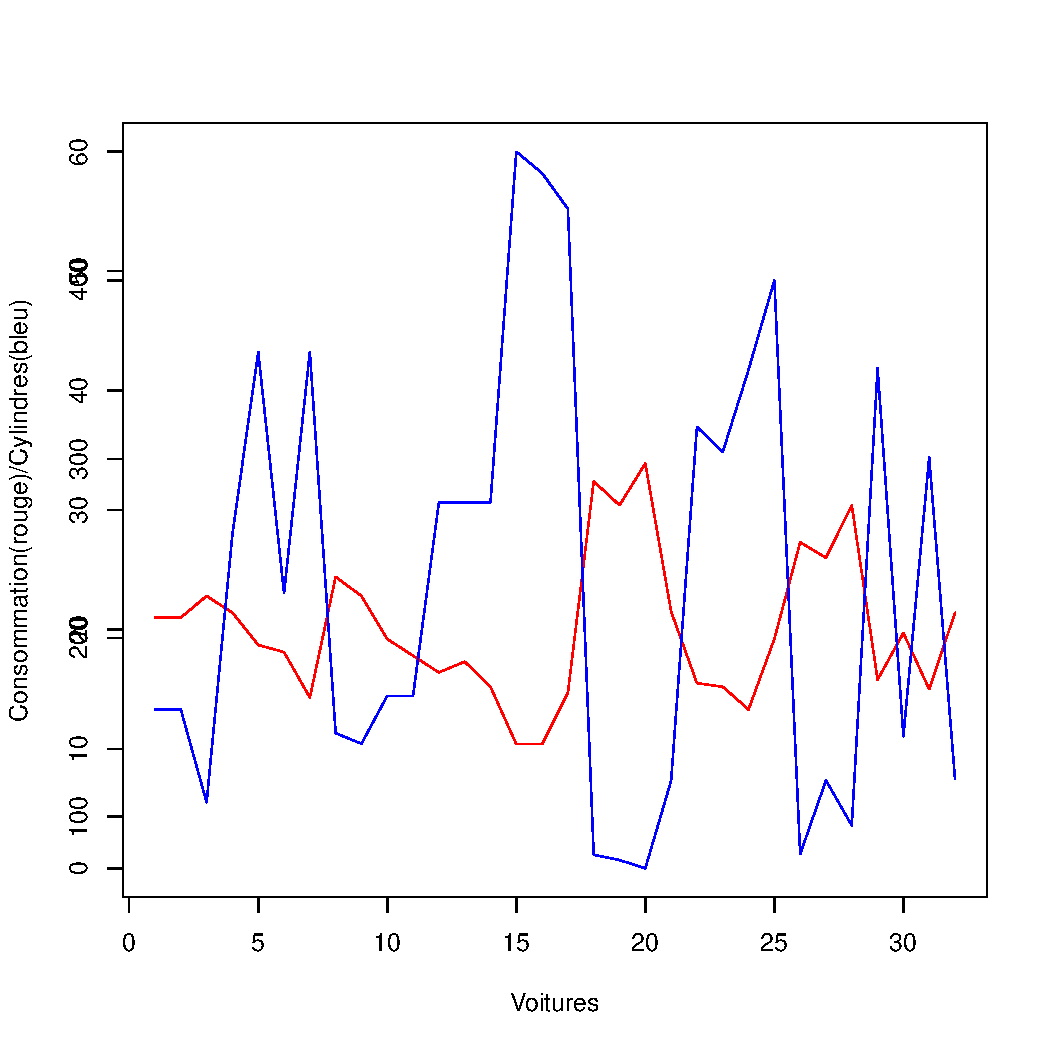
\includegraphics[scale=0.5]{graphicC.pdf}
\caption{Consommation et nombres de cylindres}
\end{figure}

Min.   :10.40\\
1st Qu.:15.43\\
Median :19.20\\
Mean   :20.09\\
3rd Qu.:22.80\\
Max.   :33.90\\

\section{Nombre de cylindres}
    
Min.   :4.000\\
1st Qu.:4.000\\
Median :6.000\\
Mean   :6.188\\
3rd Qu.:8.000\\
Max.   :8.000\\

\section{Cylindrée}
\begin{figure}[h]
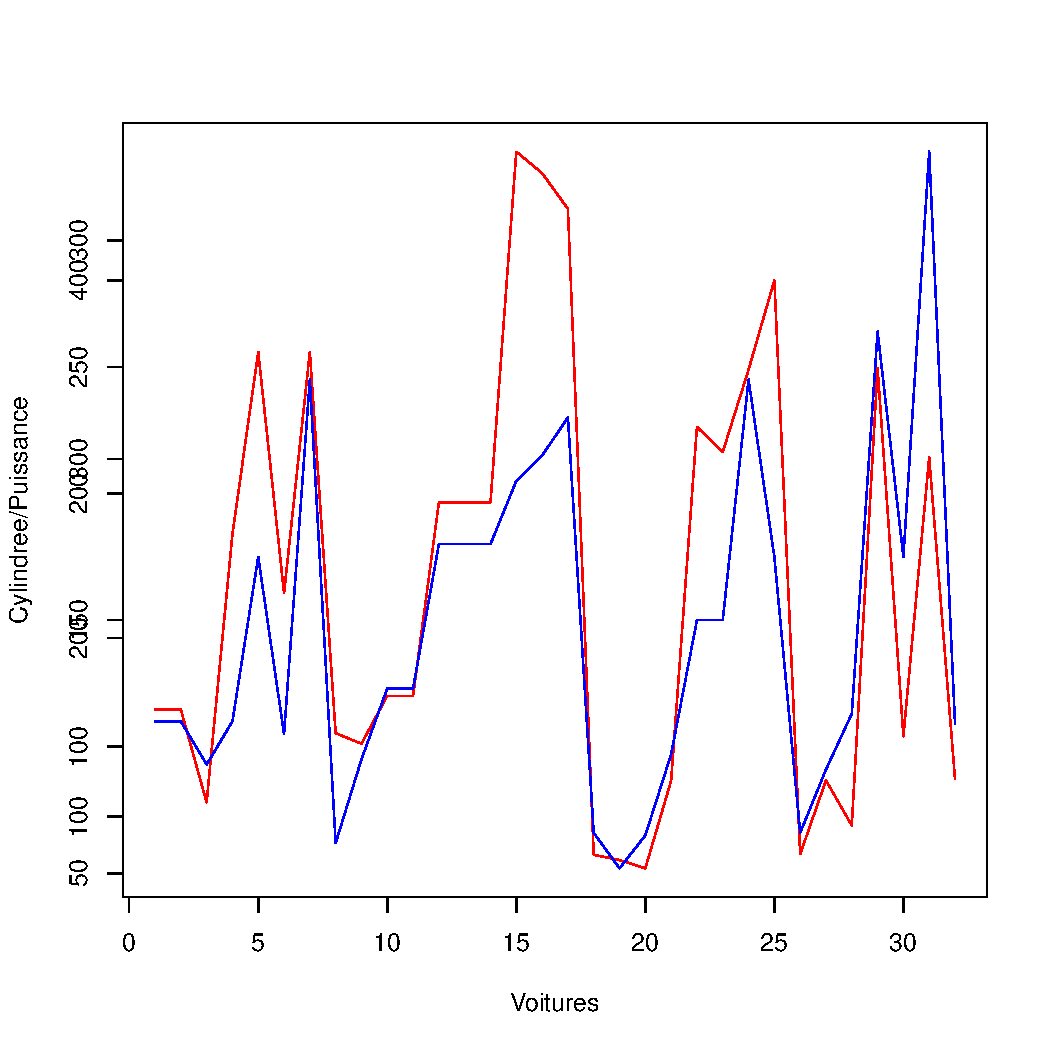
\includegraphics[scale=0.5]{graphicB.pdf}
\caption{Cylindree et Puissance}
\end{figure}
    
Min.   : 71.1\\
1st Qu.:120.8\\
 Median :196.3\\ 
Mean   :230.7\\
3rd Qu.:326.0\\
 Max.   :472.0\\

\section{Puissance}
     
Min.   : 52.0\\
1st Qu.: 96.5\\
Median :123.0\\
Mean   :146.7\\
3rd Qu.:180.0\\
Max.   :335.0\\

\section{Poids}

\begin{figure}[h]
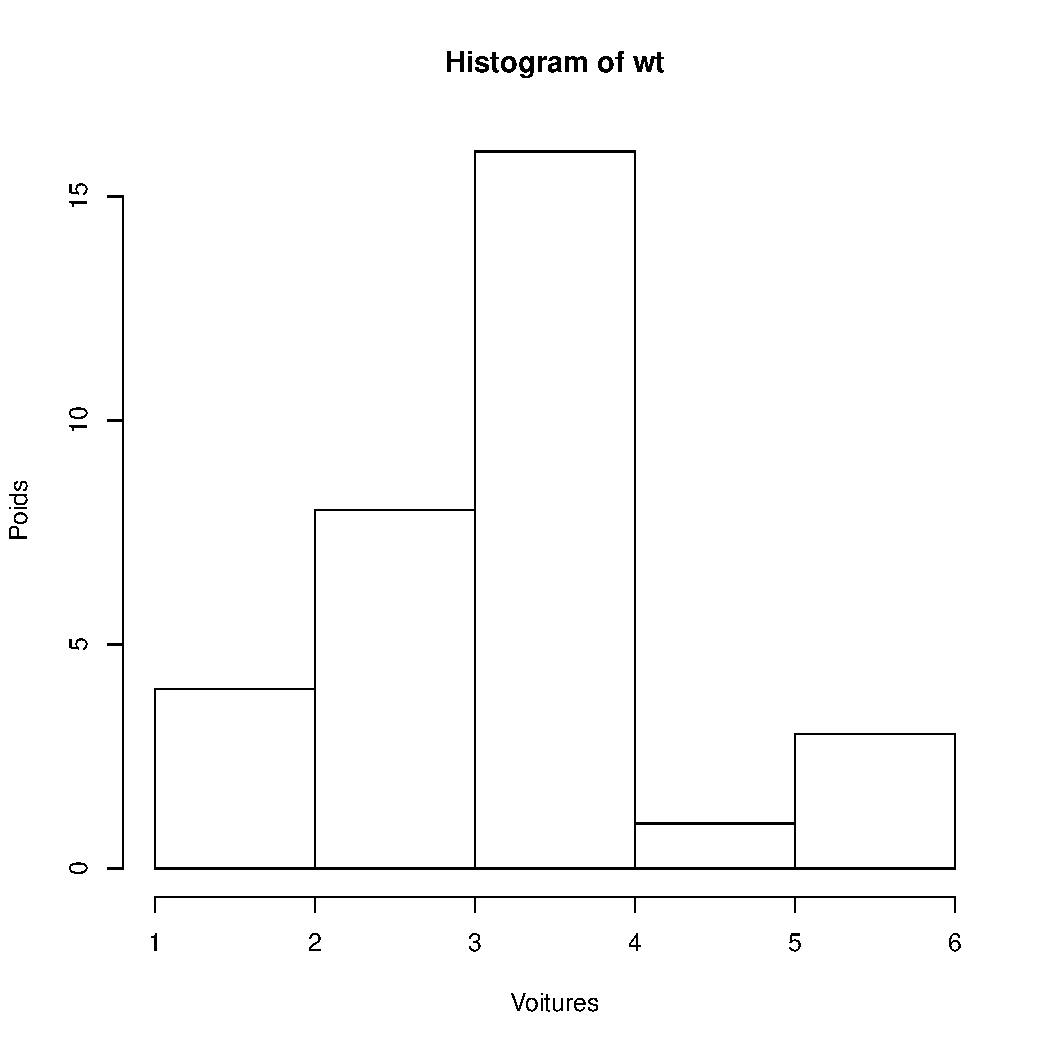
\includegraphics[scale=0.5]{graphicA.pdf}
\caption{Poids}
\end{figure}
       
Min.   :2.760\\ 
1st Qu.:3.080\\
Median :3.695\\  
Mean   :3.597\\ 
3rd Qu.:3.920\\
Max.   :4.930\\

\section{Nombre de vitesses}
 
 Min.   :0.0000\\
 1st Qu.:0.0000\\
 Median :0.0000\\
 Mean   :0.4062\\
 3rd Qu.:1.0000\\
 Max.   :1.0000\\

\begin{figure}[h]
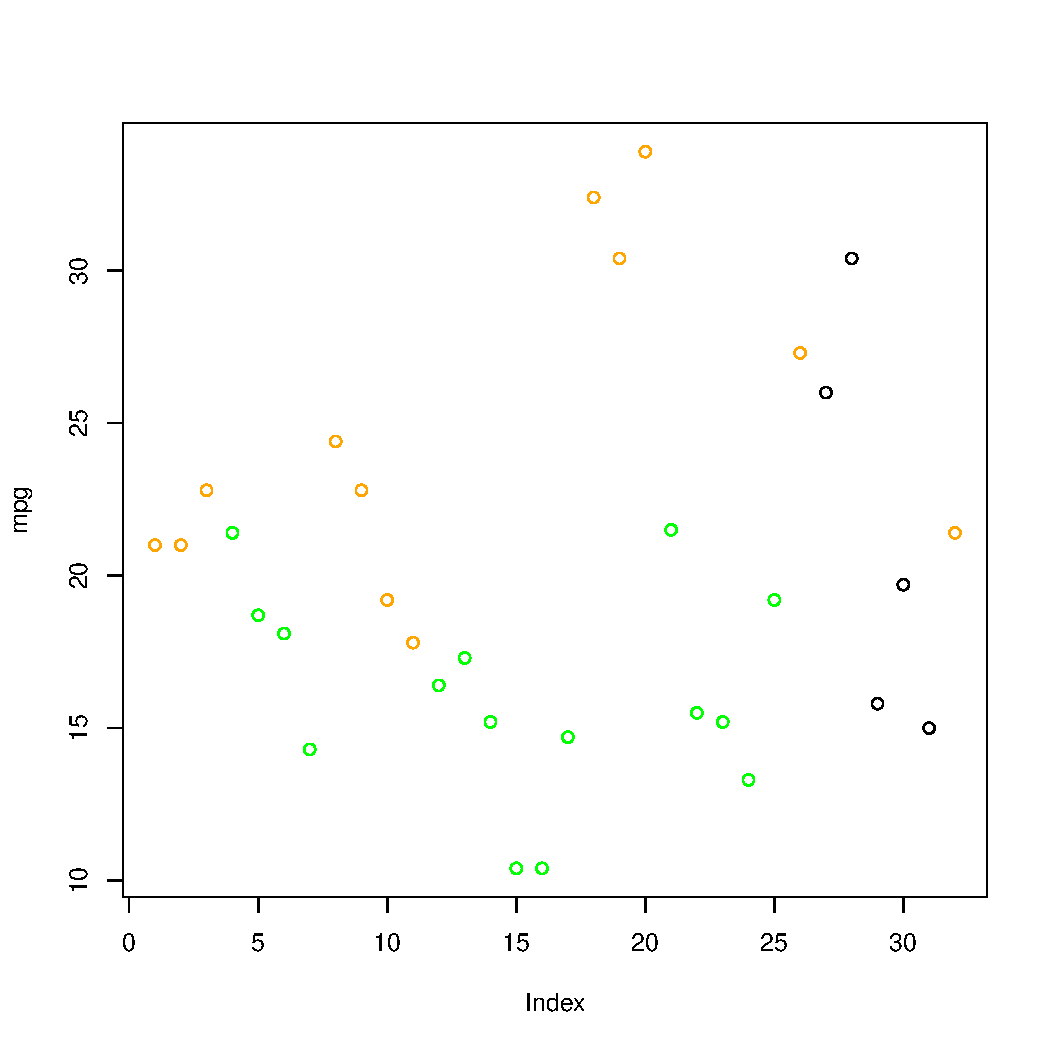
\includegraphics[scale=0.5]{graphicD.pdf}
\caption{Bilan}
\label{Bilan Du Graphique}
\end{figure}

On peut voir juste au dessus le bilan de la consommantion en fonction des différentes voitures étudiées.



\end{document}
